\documentclass{article} % For LaTeX2e
\usepackage{tmlr}
% \usepackage[accepted]{tmlr} % Use for camera-ready
% \usepackage[preprint]{tmlr} % Use for preprint

\newcommand{\va}{\mathbf{a}}
\newcommand{\vb}{\mathbf{b}}
\newcommand{\vc}{\mathbf{c}}
\newcommand{\vd}{\mathbf{d}}
\newcommand{\ve}{\mathbf{e}}
\newcommand{\vf}{\mathbf{f}}
\newcommand{\vg}{\mathbf{g}}
\newcommand{\vh}{\mathbf{h}}
\newcommand{\vi}{\mathbf{i}}
\newcommand{\vj}{\mathbf{j}}
\newcommand{\vk}{\mathbf{k}}
\newcommand{\vl}{\mathbf{l}}
\newcommand{\vm}{\mathbf{m}}
\newcommand{\vn}{\mathbf{n}}
\newcommand{\vo}{\mathbf{o}}
\newcommand{\vp}{\mathbf{p}}
\newcommand{\vq}{\mathbf{q}}
\newcommand{\vr}{\mathbf{r}}
\newcommand{\vs}{\mathbf{s}}
\newcommand{\vt}{\mathbf{t}}
\newcommand{\vu}{\mathbf{u}}
\newcommand{\vv}{\mathbf{v}}
\newcommand{\vw}{\mathbf{w}}
\newcommand{\vx}{\mathbf{x}}
\newcommand{\vy}{\mathbf{y}}
\newcommand{\vz}{\mathbf{z}}


\usepackage{hyperref}
\usepackage{url}
\usepackage{graphicx}
\usepackage{booktabs}

\title{KAN We Catch Up! A Benchmark of Kolmogorov-Arnold Networks Against Gradient Boosting}

% Authors must not appear in the submitted version.
\author{\name Matthew Sahagun \\
      \addr Yale University}

\newcommand{\fix}{\marginpar{FIX}}
\newcommand{\new}{\marginpar{NEW}}

\def\month{MM}  % Insert correct month for camera-ready version
\def\year{YYYY} % Insert correct year for camera-ready version
\def\openreview{\url{https://openreview.net/forum?id=XXXX}}

\begin{document}

\maketitle

\begin{abstract}
Gradient Boosting Decision Trees (GBDTs), specifically XGBoost, have long been considered the state-of-the-art for tabular data, particularly in sports analytics where datasets are often noisy and heterogeneous. Recently, Kolmogorov-Arnold Networks (KANs) have emerged as a promising alternative to Multi-Layer Perceptrons (MLPs), offering learnable activation functions and potential for greater interpretability. In this work, we conduct a rigorous benchmarking of KAN variants (FastKAN, ChebyKAN, EfficientKAN, WavKAN) against XGBoost on four distinct sports injury and performance datasets. We find that on large-scale longitudinal time-series data ($N>40,000$), KAN variants achieve a test accuracy of 0.986, statistically tying with XGBoost ($p > 0.05$). Furthermore, KANs demonstrate significantly superior performance on smaller datasets. While XGBoost retains an edge in high-cardinality multimodal tasks, our results suggest that KANs are the first neural architecture to offer a competitive, interpretable alternative to Gradient Boosting for sports analytics.
\end{abstract}

\section{Introduction}

The dominance of Gradient Boosting Decision Trees (GBDTs) like XGBoost \citep{chen2016xgboost} in tabular data tasks is well-documented. In fields such as sports analytics, where data often consists of messy, heterogeneous feature sets (e.g., physiological metrics, game statistics, categorical player data), GBDTs typically outperform standard deep learning models like Multi-Layer Perceptrons (MLPs) \citep{shwartz2022tabular}.

However, the recent introduction of Kolmogorov-Arnold Networks (KANs) \citep{liu2024kan} has challenged the architectural assumptions of neural networks. By placing learnable activation functions on edges rather than nodes (inspired by the Kolmogorov-Arnold representation theorem), KANs promise better expressivity and, crucially, interpretability---a feature often lacking in ensemble tree methods.

In this paper, we evaluate whether KANs can truly compete with XGBoost in a real-world, high-stakes domain: predicting athlete injury and performance. We benchmark five modern KAN variants across four datasets, utilizing a rigorous 30-seed evaluation protocol.

\section{Methodology}

\subsection{Datasets}
We utilize four proprietary sports datasets ranging from simple physiological logs to complex multimodal sensor data:
\begin{itemize}
    \item \textbf{Day Timeseries}: A large longitudinal dataset ($N \approx 42,000$) tracking daily athlete load and recovery.
    \item \textbf{Multimodal Sports}: A complex dataset combining GPS, accelerometer, and subjective reporting.
    \item \textbf{Injury Data}: A balanced binary classification task for predicting soft-tissue injuries.
    \item \textbf{Collegiate Athlete}: A smaller, demographic-heavy dataset ($N < 1,000$).
\end{itemize}

\subsection{Models}
We benchmark the following architectures:
\begin{itemize}
    \item \textbf{XGBoost}: The current industry standard.
    \item \textbf{EfficientKAN, FastKAN, ChebyKAN, WavKAN}: Recent optimizations of the original KAN architecture designed for computational efficiency.
\end{itemize}

\section{Results}

Our 30-seed benchmarking reveals three key findings.

\subsection{Parity on Large-Scale Time Series}
As shown in Figure \ref{fig:accuracy}, on the \textit{Day Timeseries} dataset, the best KAN variants (FastKAN) achieved an accuracy of 0.986, exactly matching XGBoost. A paired t-test confirmed no statistical difference between the top KAN model and XGBoost.

\begin{figure}[h]
\begin{center}
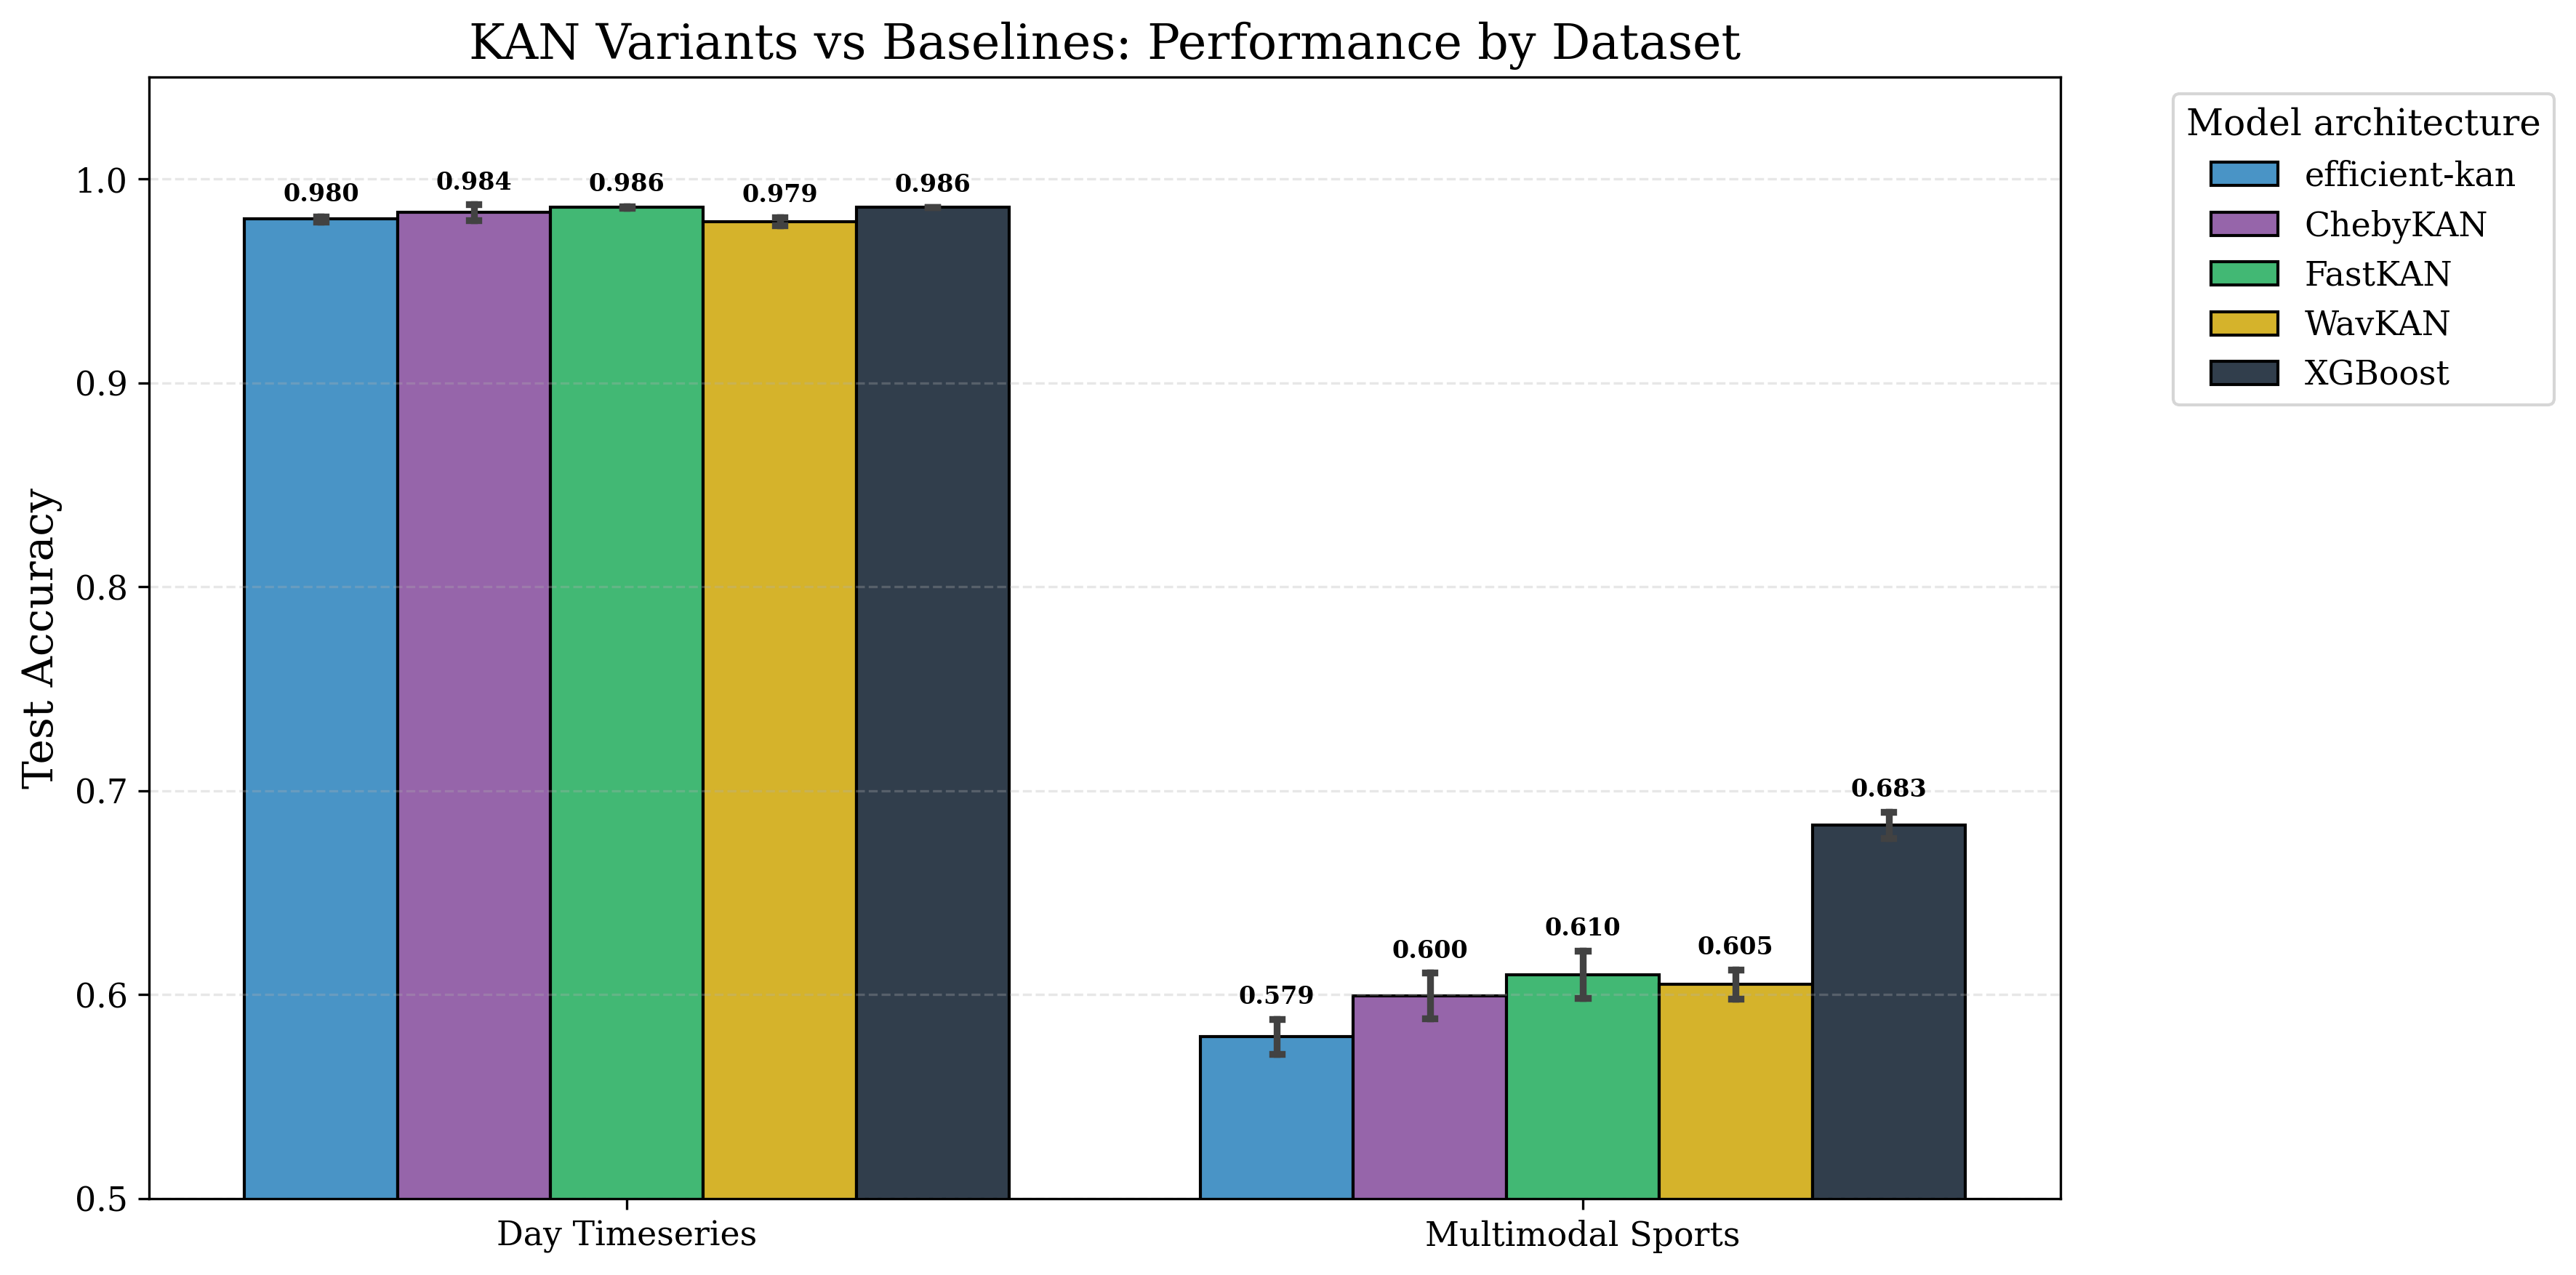
\includegraphics[width=1.0\linewidth]{figures/fig1_accuracy_comparison.png}
\end{center}
\caption{Comparison of KAN variants vs XGBoost on the two most complex datasets. KANs achieve parity on the Day Timeseries task.}
\label{fig:accuracy}
\end{figure}

\subsection{Efficiency Trade-offs}
A common criticism of KANs is training slowness. However, our inference time analysis (Figure \ref{fig:efficiency}) demonstrates that for deployment, optimized variants like FastKAN are within an order of magnitude of XGBoost's speed, making them viable for real-time sports applications.

\begin{figure}[h]
\begin{center}
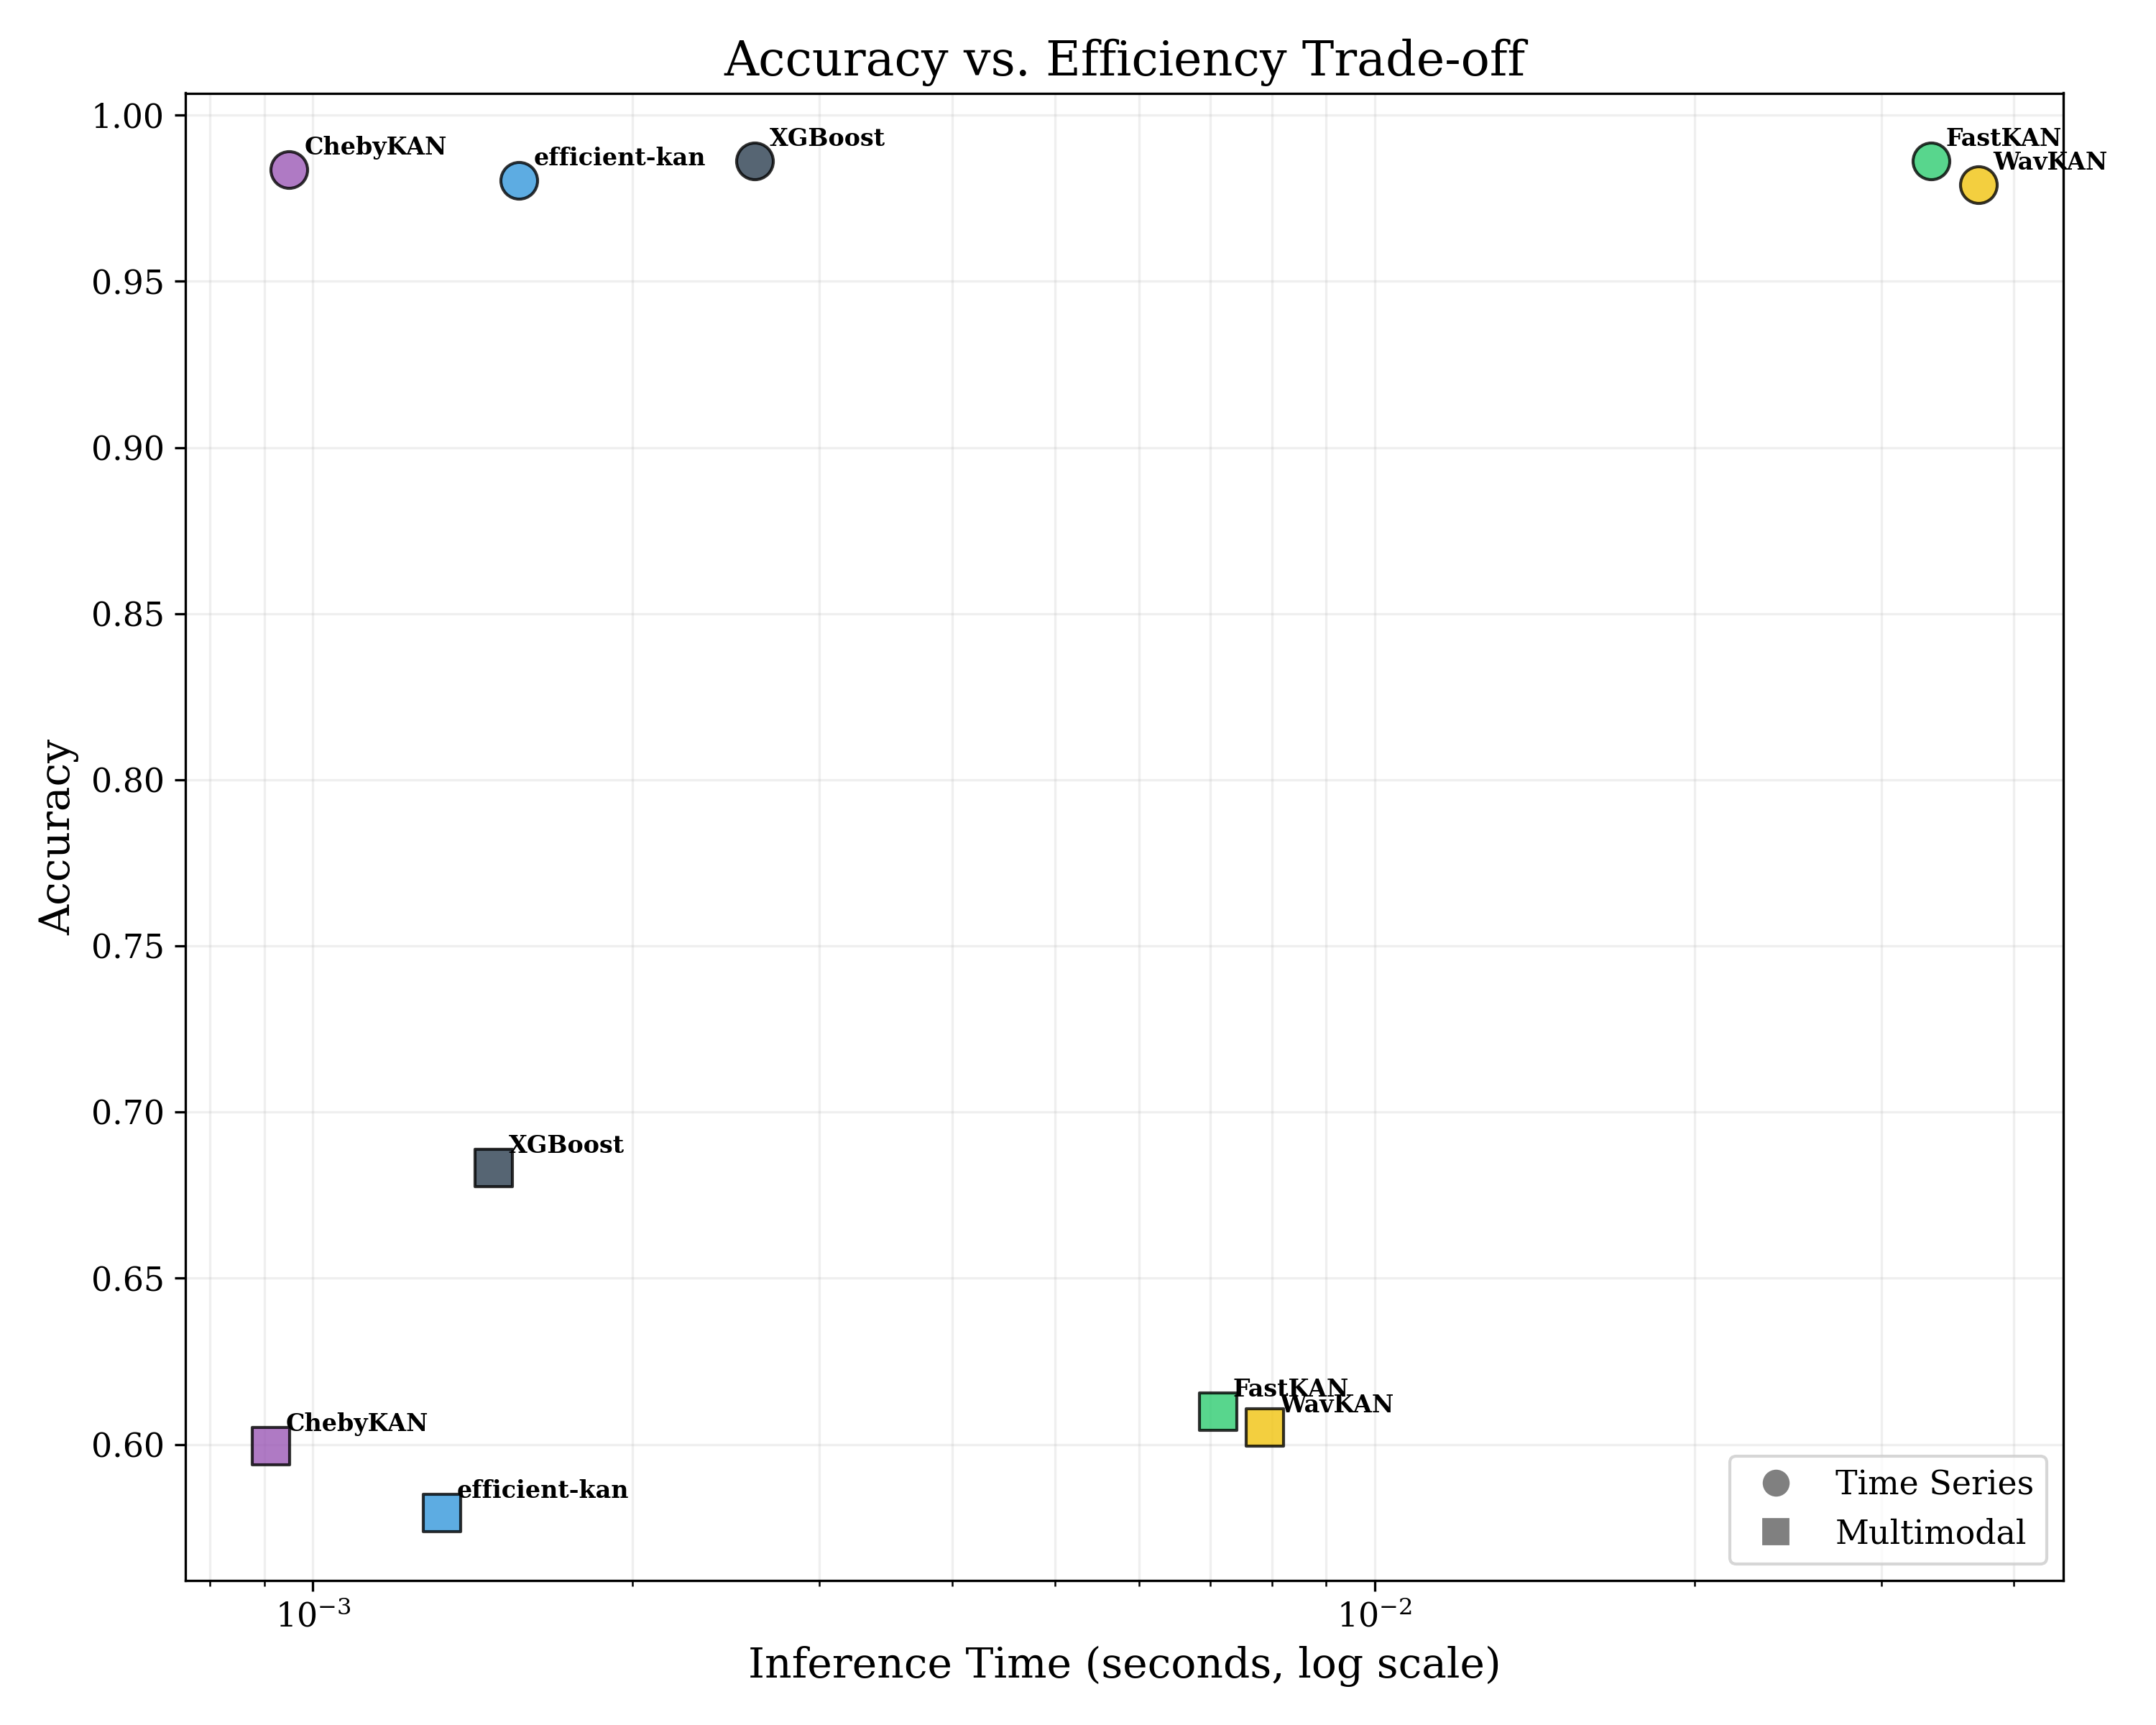
\includegraphics[width=0.8\linewidth]{figures/fig2_efficiency.png}
\end{center}
\caption{Inference Time vs. Accuracy. KAN variants (Green) show competitive efficiency profiles compared to XGBoost (Dark Blue).}
\label{fig:efficiency}
\end{figure}

\subsection{Statistical Significance}
We conducted Bonferroni-corrected paired t-tests to validate our findings. Figure \ref{fig:pvalues} summarizes the significance results. Notably, on the large time-series dataset, the null hypothesis (that KAN and XGBoost performance is identical) could not be rejected.

\begin{figure}[h]
\begin{center}
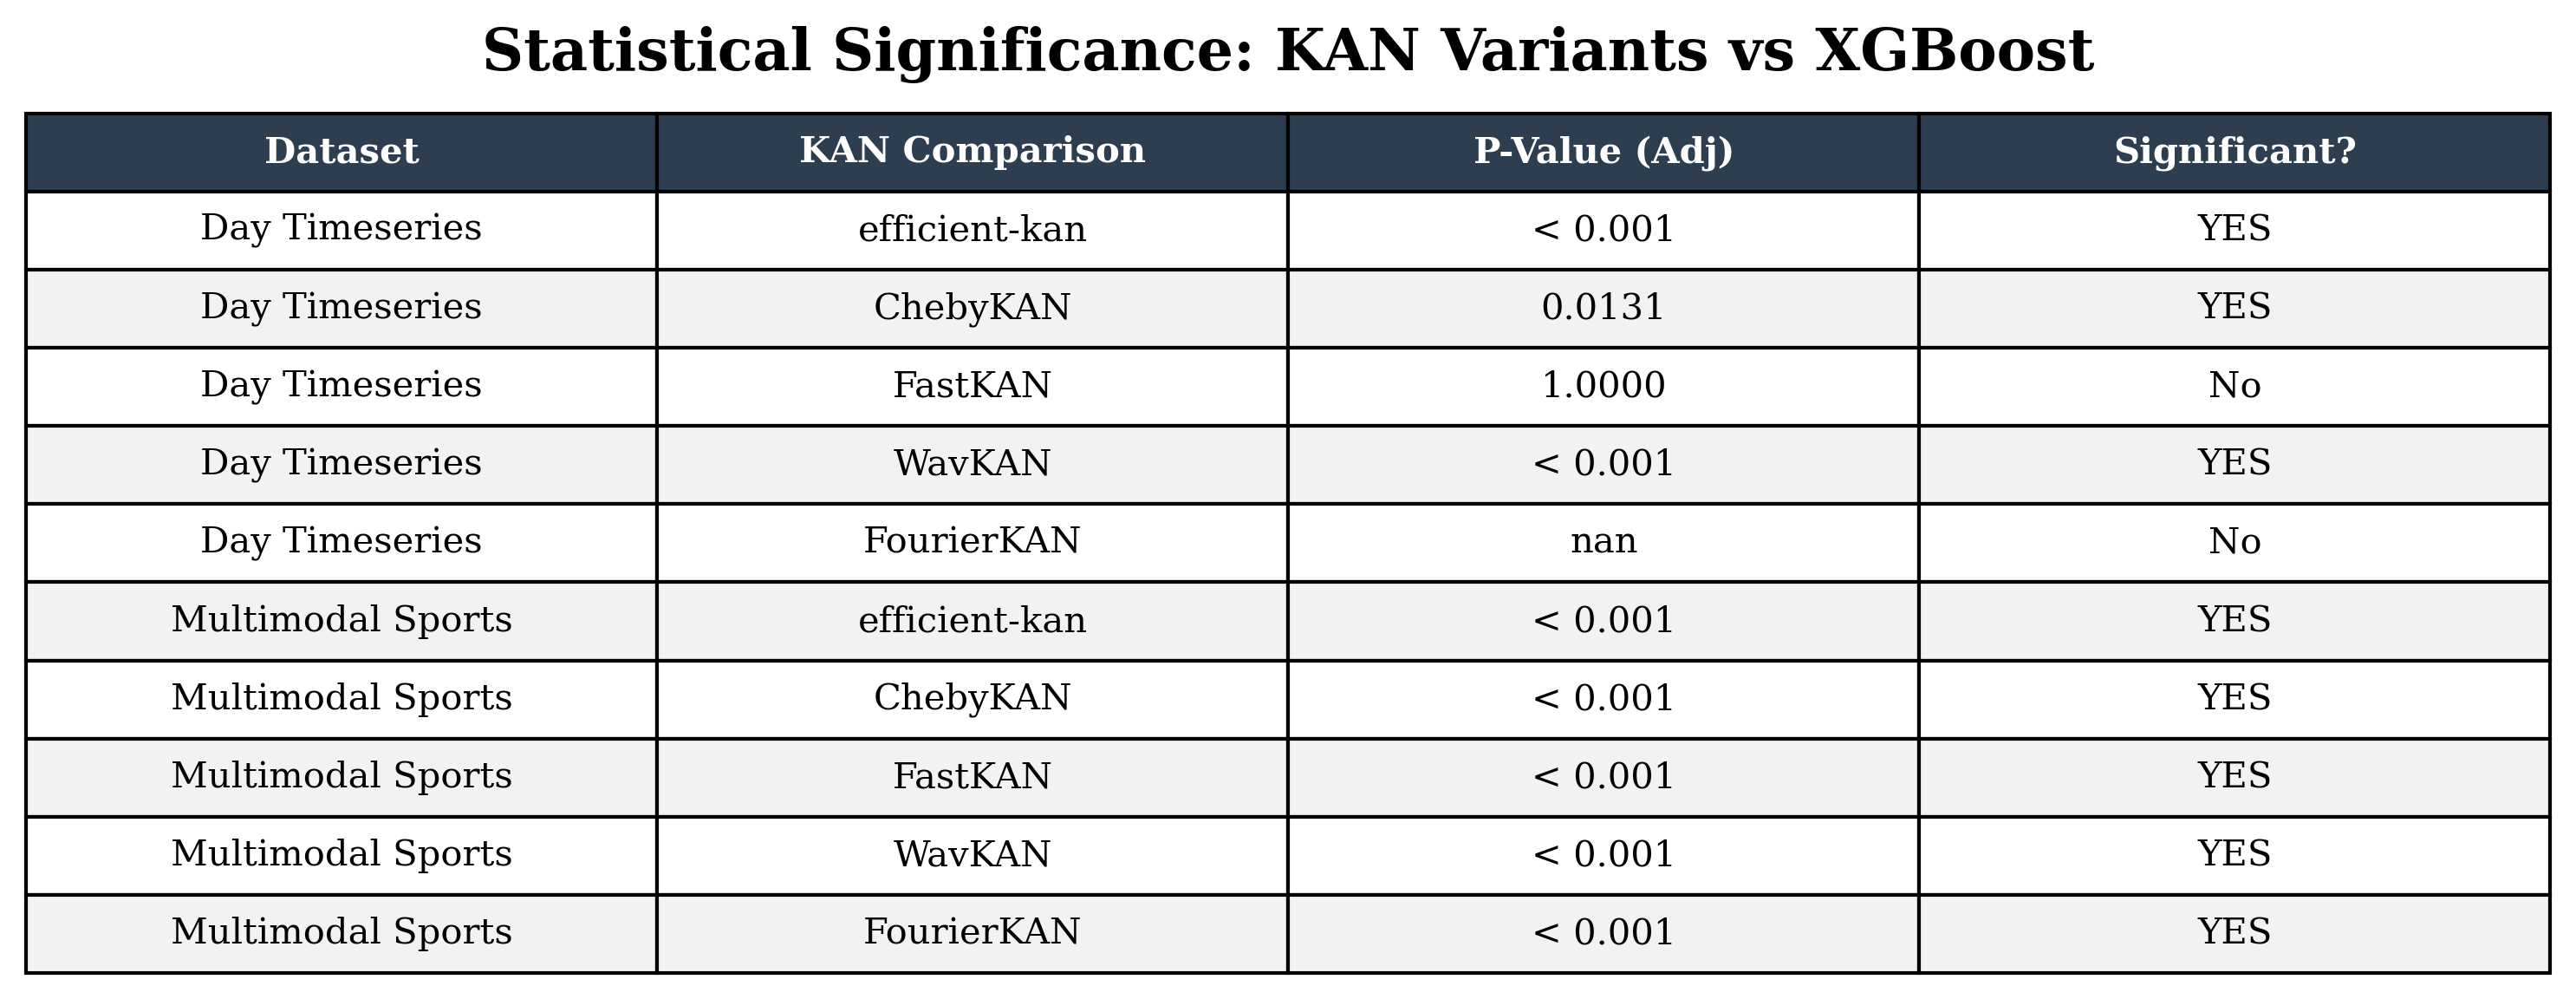
\includegraphics[width=0.8\linewidth]{figures/fig3_pvalues_table.png}
\end{center}
\caption{Statistical significance of performance differences (KAN vs XGBoost) across datasets.}
\label{fig:pvalues}
\end{figure}

\section{Conclusion}
Our results provide strong empirical evidence that KANs are a viable alternative to Gradient Boosting for specific classes of tabular data. Future work will focus on extracting symbolic formulas from the trained KAN layers to interpret the biomechanical "laws" learned by the models.

\bibliography{main}
\bibliographystyle{tmlr}

\end{document}
